\chapter{The Envelope Tool}

The MAUS envelope tool is intended as a tool to support lattice development and
enable visualisation of the MICE accelerator for online use. The tool 
facilitates the visualisation of field elements, propagation of particles and
beams ellipses through those elements.

The envelope tool is intended for use with mostly straight beamlines.

\section{Example Usage}
To call the envelope tool with some example data, source the MAUS environment 
and then do

\begin{verbatim}
$ python ${MAUS_ROOT_DIR}/bin/utilities/envelope_tool/envelope_tool.py \
  --configuration_file ${MAUS_ROOT_DIR}/bin/utilities/envelope_tool/share/pseudobeamline.py
\end{verbatim}

\begin{figure}[!htb]
\centering
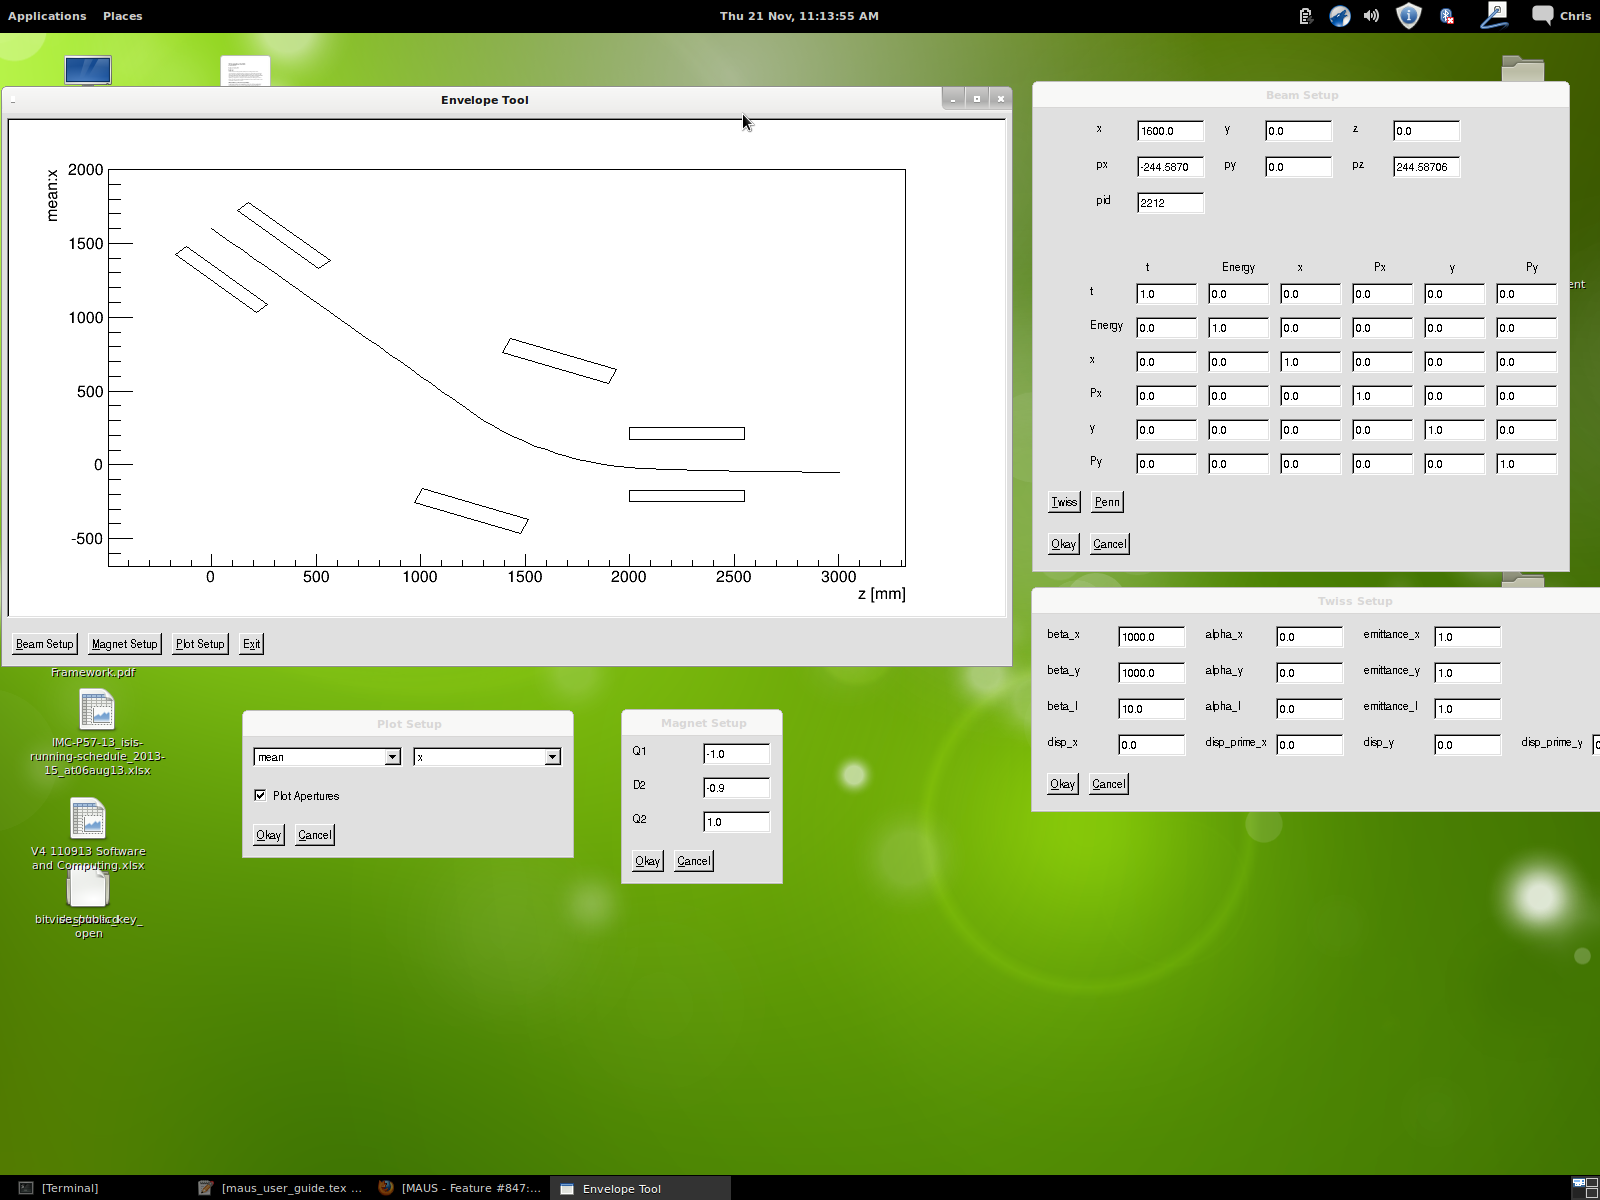
\includegraphics[width=0.9\textwidth]{envelope_tool.png}
\caption{The Envelope Tool used to plot a reference trajectory through a few magnets.}
\end{figure}

\section{Envelope Tool main window}
The Main Window enables the user to view the selected lattice parameters, and
provides buttons to update the beam, lattice and plot parameters.

\begin{itemize}
\item Beam Setup: setup a beam
\item Magnet Setup: setup fields
\item Plot Setup: setup the plot
\item Exit: exit the GUI
\end{itemize}

\section{Beam Setup}

The Beam Setup window enables the user to set beam parameters. The top few cells
set initial position, momentum and particle type of the beam centroid, also
referred to as the `reference particle' or `reference trajectory'. The bottom
few cells set beam ellipse parameters.

Helper windows can be accessed to parameterise the beam ellipse using either a
Penn parameterisation or a
Twiss parameterisation.

\begin{itemize}
\item x, y, z: initial position of the beam particle
\item px, py, pz: initial momentum of the beam particle
\item pid: PDG ID of the beam particle. This is an integer; see Tab. 
\ref{tab:pdg_id} for some common particle ids.
\item ellipse elements: set the elements of the beam ellipse.The matrix must
be symmetric and positive definite or an error will be returned when Okay is
pressed.
\item Twiss: setup the beam using a Twiss parameterisation - beam asymmetric in
x and y with no coupling
\item Penn: setup the beam using a Penn parameterisation - beam cylindrically 
symmetric in x and y with angular momentum
\item Okay: click okay to return to the main window, updating the beam ellipse
\item Cancel: click cancel to return to the main window, losing changes
\end{itemize}

\section{Magnet Setup}
The user can manipulate magnet parameters in this window. When the window is
opened, MiceModules which have the following required parameters are added to
the window.

\begin{itemize}
\item FieldType (string)
\item FieldName (string)
\item Position (hep three vector)
\item Rotation (hep three vector)
\item ScaleFactor (double)
\item NominalAperture (hep three vector)
\item NominalOuter (hep three vector)
\end{itemize}

Other MiceModules will be ignored.

Each magnet is labelled with the magnet FieldName and a text entry is available
to set the scale factor (proportional to field).

\begin{itemize}
\item <field entries>: Enter a float to set the scale factor.
\item Okay: Update the fields in the lattice
\item Cancel: Cancel changes
\end{itemize}

\section{Plot Setup}
The Plot Setup window enables the user to select the desired plot parameters.

\begin{itemize}
\item Plot Type: Select the type of variable to plot.
\item Plot Variable: Select the variable to plot.
\item Plot Apertures: tick to plot physical apertures. If the plot type is
\verb|mean| or \verb|envelope| and plot variable is \verb|x| or \verb|y| the 
apertures will be 
plotted as a 2D projection of the physical apertures in the appropriate plane,
with the beam reference trajectory or beam envelope superimposed. Note that the
rotations applied here are rather simplistic, assuming a 2D geometry in x or y
plane (but not both) Otherwise nominal apertures will be scaled to fit in the 
upper portion of the plotting window.
\item Okay: Update the plot in the main window with the new selection.
\item Cancel: Cancel changes
\end{itemize}


